\chapter{Mengenal Python dan Anaconda}
Tujuan pembelajaran pada pertemuan pertama antara lain:
\begin{enumerate}
\item
Mengerti sejarah python, perkembangan dan penggunaan python di perusahaan
\item
Memahami tahapan instalasi python dan anaconda
\item
Memahami cara penggunaan spyder
\end{enumerate}
Tugas dengan cara dikumpulkan dengan pull request ke github dengan menggunakan format latex pada repo yang dibuat oleh asisten IRC.

\section{Teori}
Praktek teori penunjang yang dikerjakan :
\begin{enumerate}
\item
Buat Resume Sejarah Python, perbedaan python 2 dan 3, dengan bahasa yang mudah dipahami dan dimengerti. Buatan sendiri bebas plagiat(10)
\item
Buat Resume Implementasi dan penggunaan Python di perusahaan dunia, bahasa yang mudah dipahami(10)
\end{enumerate}

\section{Instalasi}
Melakukan instalasi python dan anaconda versi 3 serta uji coba spyder. Dengan menggunakan bahasa yang mudah dimengerti dan bebas plagiat. 
Dan wajib skrinsut dari komputer sendiri.
\begin{enumerate}
\item
Instalasi python 3 (5)
\item
instalasi pip(5)
\item
cara setting environment (5)
\item
mencoba entrepreter/cli melakui terminal atau cmd windows(5)
\item 
Menjalankan dan mengupdate anaconda dan spyder(5)
\item
Cara menjalankan Script hello word di spyder(5)
\item
Cara menjalankan Script otomatis login aplikasi akademik dengan library selenium dan inputan user(5)
\item
Cara pemakaian variable explorer di spyder(5)
\end{enumerate}


\section{Identasi}
Membuat file main.py dan mengisinya dengan script contoh python penggunaan selenium(minimal 20 baris) yang melibatkan inputan user, kemudian mencoba untuk mengatasi error identasi.
\begin{enumerate}
	\item
Penjelasan Identasi (10)
	\item
jenis jenis error identasi yang didapat(10)
\item
cara membaca error(10)
\item 
cara menangani errornya(10)
\end{enumerate}

\section{Presentasi Tugas}
Pada pertemuan ini, diadakan tiga penilaiain yaitu penilaian untuk tugas mingguan dengan nilai maksimal 100. Kemudian dalam satu minggu kedepan maksimal sebelum waktu mata kuliah. Ada presentasi kematerian dengan nilai presentasi yang terpisah masing-masing 100. Dan nilai terpisah untuk tutorial dari jawaban tugas di YouTube.Jadi ada tiga komponen penilaiain pada pertemuan ini yaitu :
\begin{enumerate}
	\item tugas minggu hari ini dan besok (maks 100). pada chapter ini
	\item presentasi csv (maks 100). Mempraktekkan kode python dan menjelaskan cara kerjanya.
	\item pembuatan video tutorial youtube tentang tutorial dari jawaban tugas.(nilai maks 100)
\end{enumerate}
Waktu presentasi pada jam kerja di IRC. Kriteria penilaian presentasi sangat sederhana, presenter akan ditanyai 20(10 pertanyaan program, 10 pertanyaan teori) pertanyaan tentang pemahamannya menggunakan python dan program agan dibuat error hingga presenter bisa menyelesaikan errornya. jika presenter tidak bisa menjawab satu pertanyaan asisten maka nilai nol. Jika semua pertanyaan bisa dijawab maka nilai 100. Presentasi bisa diulang apabila gagal, sampai bisa mendapatkan nilai 100 dalam waktu satu minggu kedepan.

\section{Jawaban Teori}
\begin{enumerate}
    \item Python adalah bahasa pemrograman interpretatif multiguna dengan filosofi perancangan yang berfokus pada tingkat keterbacaan kode. Python diklaim sebagai bahasa yang menggabungkan kapabilitas, kemampuan, dengan sintaksis kode yang sangat jelas, dan dilengkapi dengan fungsionalitas pustaka standar yang besar serta komprehensif. perbedaan phython2 dan 3 adalah python 2 dan 3 memiliki beberapa hal yang menjadi  perbedaan antar versinya. kenapa tiap versi berbeda karena setiap produk akan terus memperbaiki dan mengoptimalkan fitur — fitur yang ada demi terwujudnya produk yang efektif seperti tampilan file print berbeda, modul future yanf berbeda
    
    \item  layanan musik streaming Spotify memanfaatkan Python untuk membuat analisis data dan backend. backend Spotify banyak terdapat service yang berkomunikasi lewat 0MQ (ZeroMQ) yang merupakan framework dan library open source untuk networking. 0MQ dibuat menggunakan Python dan C++. Alasan service dibuat menggunakan Python dikarenakan Spotify sangat menyukai kecepatan pipeline development. Sistem rekomendasi Spotify bergantung pada analisis data yang sangat besar, untuk menginterpretasikan analisis tersebut Spotify menggunakan Luigi, modul Python yang sinkron dengan Hadoop. Modul open source ini menangani satu library dengan library lainnya agar saling bekerjasama, dan mengkonsolidasi eror log secara cepat.

\end{enumerate}




\section{Jawaban Instalasi}

\begin{enumerate}
\item   Instalasi PYHTON
    \begin{enumerate}
   \item \noindent
   Setelah download selesai, kita akan mendapatkan file python-3.4.2.msi.File  akan melakukan instalasi ke sistem windows.
    \begin{center}
            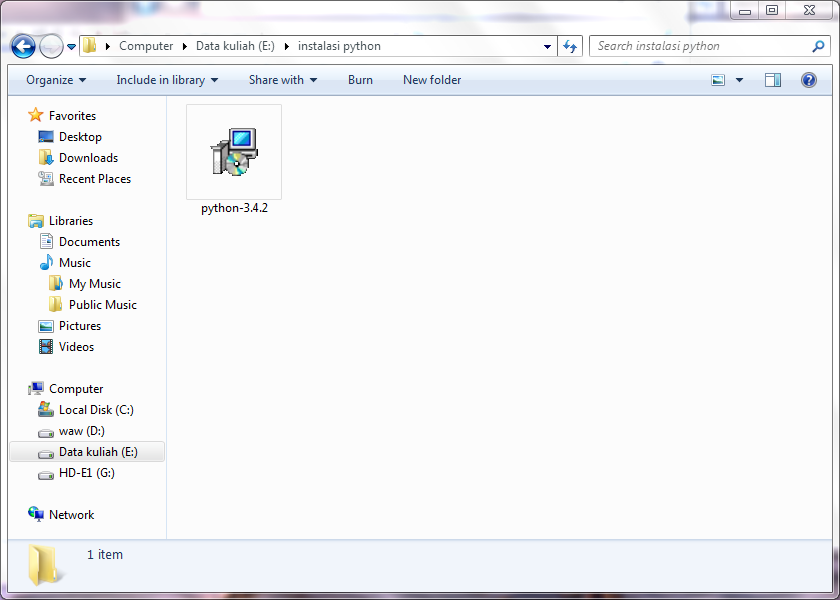
\includegraphics[width=10cm]{figures/1.png}
        \end{center}
    \item
    akan muncul kotak dialog.Pilih Install For All Users. Kemudian klik Next.
   \begin{center}
            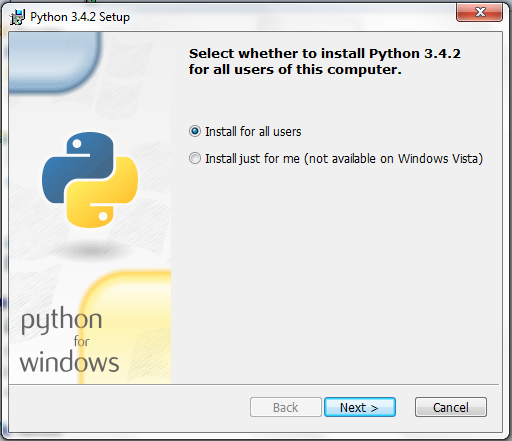
\includegraphics[width=10cm]{figures/2.PNG}
        \end{center}
    \item kotak dialog kostumisasi Python, scroll ke bawah, dan pilih Add Python.exe to path. Pilih Will be installed on local hardrive. Klik Next.
   \begin{center}
            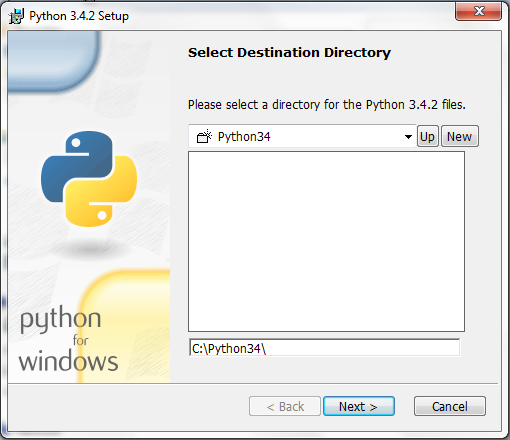
\includegraphics[width=10cm]{figures/3.PNG}
        \end{center}
   \item Tunggu sampai proses instalasi selesai.
 \begin{center}
            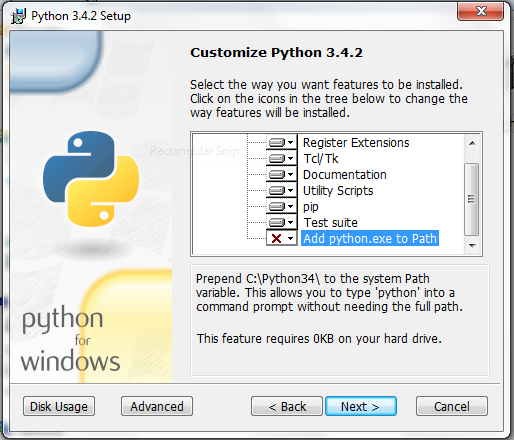
\includegraphics[width=10cm]{figures/4.PNG}
        \end{center}
    \item Bila sudah selesai, akan keluar kotak dialog sebagai berikut. Hal ini menandakan bahwa python sudah terinstal di komputer dan sudah siap untuk digunakan. Klik Finish.
 \begin{center}
            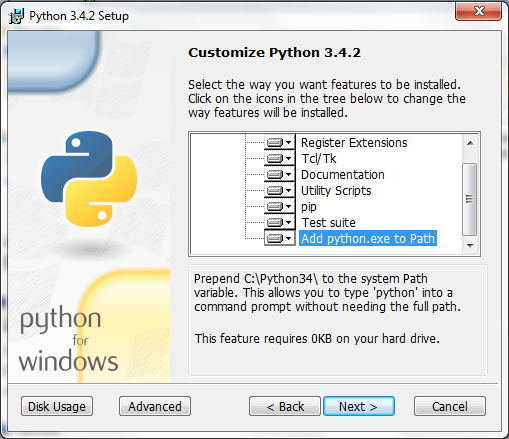
\includegraphics[width=10cm]{figures/5.PNG}
        \end{center}
    \end{enumerate}  
    
      
    `\item Instalasi PIP
    
    Pengertian PIP
    
    PIP merupakan Package Management System yang digunakan untuk mengunduh dan mengelola package Python. Dengan menggunakan pip kita dapat dengan mudah mengunduk paket-paket atau modul-modul Python
        \begin{enumerate}
    1.Instal file get-pip.py tersebut dengan cara membuka file dengan Python.exe atau dengan cara menjalankan dengan command prompt ketikan pertintah python get-pip.py yang dijalankan dalam folder yang terdapat file get-pip.py berjalan.
    \begin{center}
            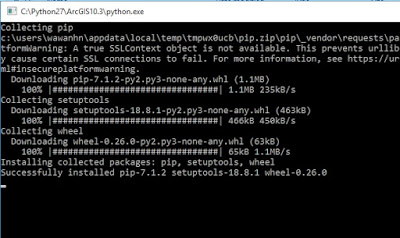
\includegraphics[width=10cm]{figures/pip1.jpg}
        \end{center}
    
    
    2.set PATH dalam environmental variabel ke tempat dimana pip.exe berada, menggunakan Python bawaan dari ArcGIS lokasi path tersebut di C:Python27 ArcGIS10.3 Scripts. Namun jika menginstal Python secara manual  pathnya berada di C: Python27 Scripts.
    \begin{center}
            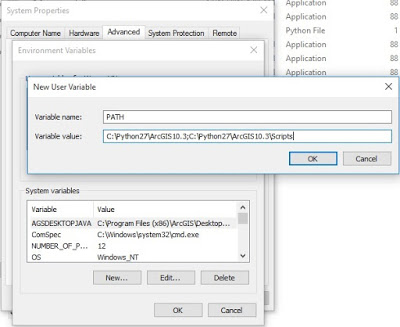
\includegraphics[width=10cm]{figures/pip2.jpg}
        \end{center}
    
    
    3.Untuk mengecek instalasi pip apakah berhasil dilakukan di komputer kita ketika perintah pip id command prompt.
    \begin{center}
            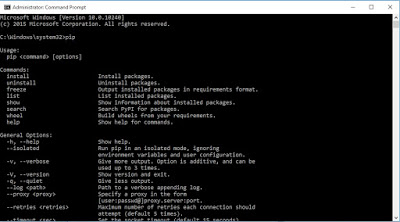
\includegraphics[width=10cm]{figures/pip3.jpg}
        \end{center}
    
        \end{enumerate}
    
    
      
      
\item Cara Setting Environment
    \begin{enumerate}
        \item  Masuk ke system pada Control Panel
        \item Control Panel System and Security System
        \item Kemudian klik  “Advanced system settings“
        \item Lanjut klik “Environment Variables” maka akan muncul lagi pop up “Environment Variables”
        \item Pada bagian System variables, scroll sampai ketemu Path. (Path adalah nama Variable)Capture007
        \item Seleksi/klik Path dan kemudian klik Edit
        \item  Maka akan muncul lagi pop up “Edit System variable”
        \item sebelum mengedit Variable value bikin dulu backup untuk mencegah hal2 yang diluar dugaan ,buka         notepad copy semua Variable value.
        \item Pada bagian paling kanan/ujung “Variable value”
        \item tambahkan path  “;C: Python36 ”  tanpa tanda petik dan klik OK pada jendela Edit System variable.
        \item klik OK pada jendela Environment Variables.
        \item klik OK pada jendela System Properties.dan close Control Panel
        \item keterangan : angka 36 pada “;C: Python36 ”adalah versi python yang saya gunakan harus disesuaikan dengan versi yang kamu download.
    \end{enumerate}
  
\item Entreprenter/Cli Melalui Terminal atau cmd Windows
    
    \begin{enumerate}
    \item ls – Command ini digunakan untuk menampilkan seluruh file dan direktori.  dengan opsi -l, sehinga akan mejadi ls -l, agar seluruh file ditampilkan dengan rapi dan disertai dengan informasi detail tentang masing-masing file tersebut
    
    \item cd – Perintah ini digunakan untuk “berjalan” diantara direktori (cd merupakan singakatan dari “change directory”). menampilkan semua file dan direktori dengan ls, memilih direktori yang ingin di jalani. , direktori home yang ingin di masuki. Masukkan perintah cd home dan Anda akan berpindah dari lokasi Anda saat ini ke direktori “home“.
    
    \item mkdir – Perintah ini digunakan untuk membuat sebuah direktori baru (merupakan singkatan dari “make directory”). Perintah ini akan membuat sebuah direktori baru dengan nama yang Anda tentukan, misalnya mkdir FolderBaru akan membuat sebuah direktori baru dengan nama FolderBaru di dalam direktori Anda berada saat ini.
    
    \item touch – Perintah ini digunakan untuk membuat sebuah file baru dengan ekstensi tertentu. Sebagai contoh, touch FileBaru.txt akan membuat sebuah file “txt” bernama FileBarudi dalam direktori 
    
    \item rm – Perintah ini digunakan untuk menghapus file/direktori tertentu. Misalnya, rm FileBaru akan menghapus file FileBaru yang sudah kita buat sebelumnya.
  
    \item cat – Perintah ini digunakan untuk menampilkan isi dari file. contoh, cat info.txt akan memunculkan isi dari file tersebut ke layar cmd.
    
    \item pwd – Perintah ini akan menampilkan lokasi Anda saat ini dalam sistem. Misalnya, ketikkan pwd, maka hasilnya adalah: “home/user/public html”.
    
    \item cp – Perintah ini digunakan untuk meng-copy file dan folder. Perintahnya adalah: cp [opsi] sumber tujuan. Pada dasarnya, Anda bisa mengetikkan langsung file yang ingin Anda copy di bagian source. 
    \end{enumerate}
    
\item Menjalankan Dan Mengupdate anaconda dan spyder
    \begin{enumerate}
        \item 
    \end{enumerate}
    
\item MenampilKan helloword di spyder
    \begin{enumerate}
        \item pertama buka aplikasi anaconda navigator di windows 10
         \begin{center}
            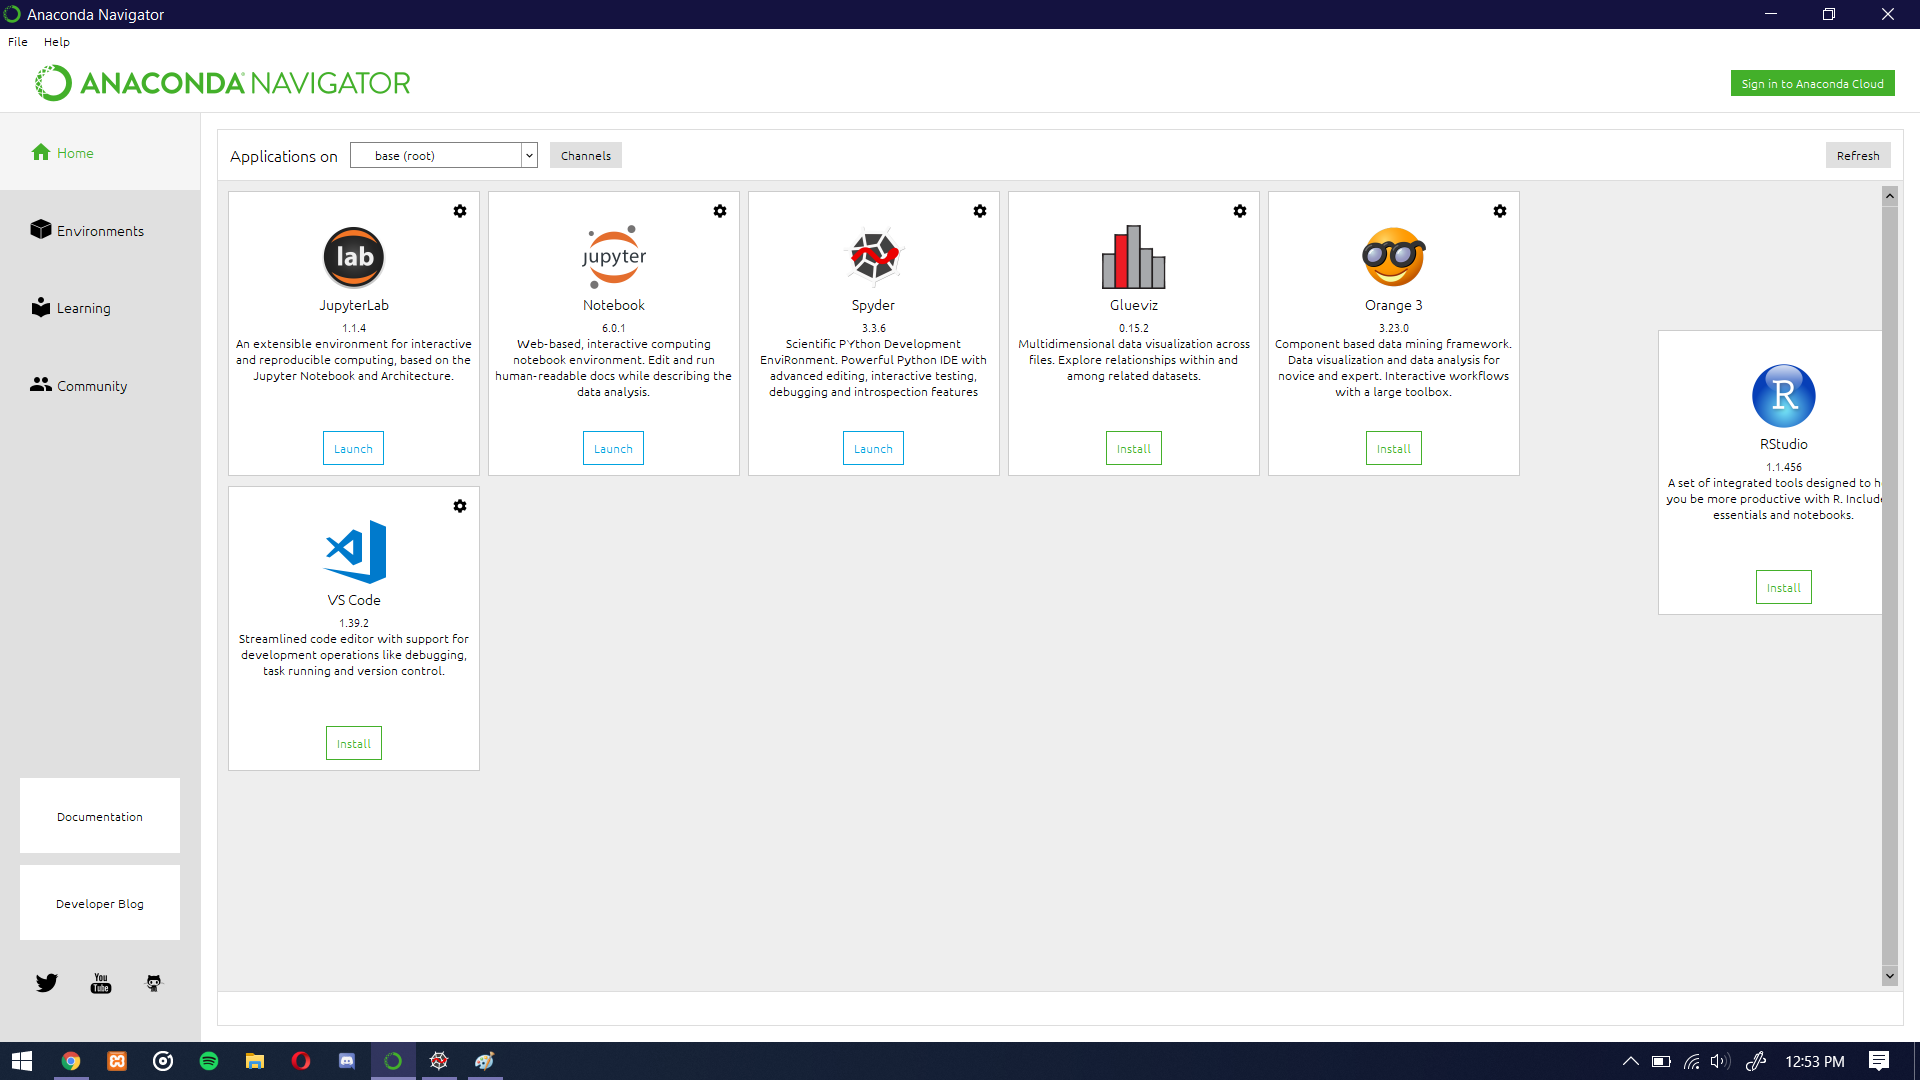
\includegraphics[width=10cm]{figures/Hw.PNG}
        \end{center}
        \item ketikan print ("HELLO WORD") di aplikasi spider untuk menampilkan kodingan yang telah di ketik
         \begin{center}
            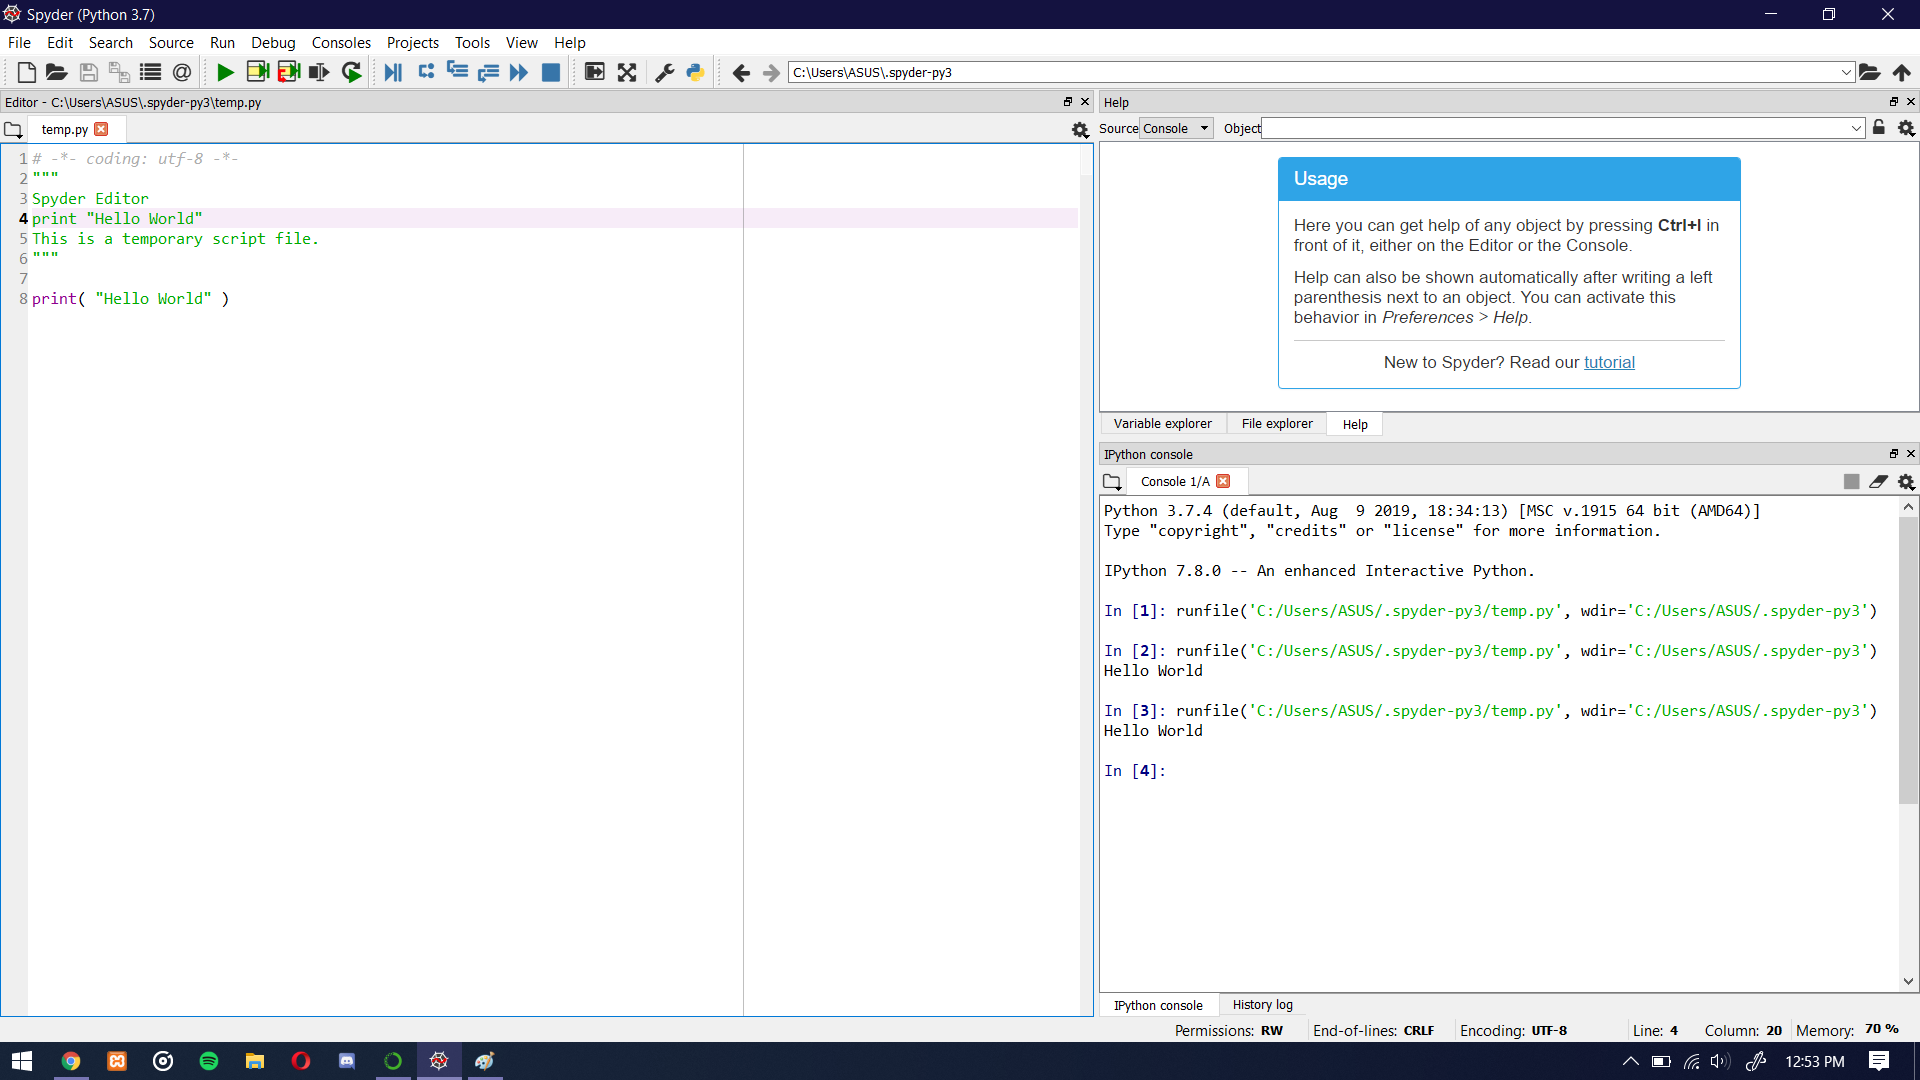
\includegraphics[width=10cm]{figures/Hw1.png}
        \end{center}
    \end{enumerate}
\item Cara Pemakaian Variable Explorer Di Spyder

 \begin{center}
            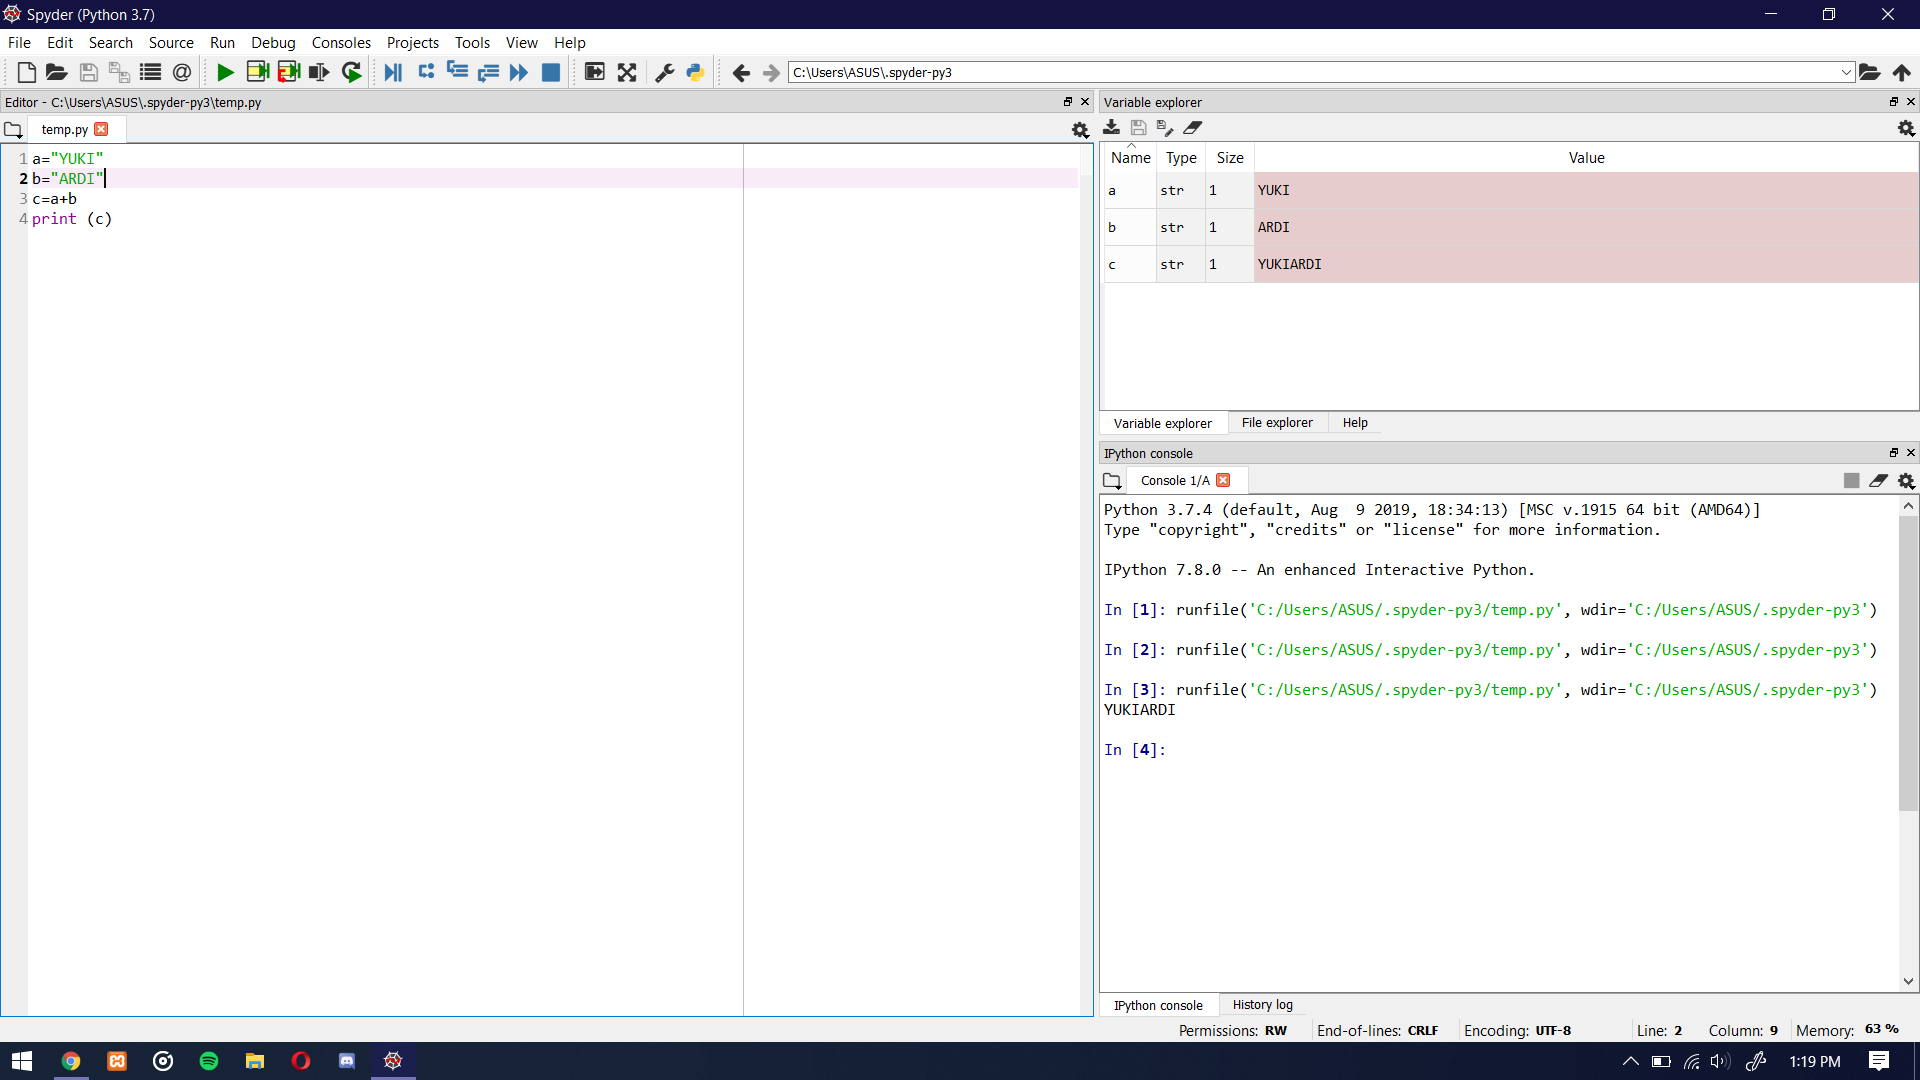
\includegraphics[width=10cm]{figures/8.png}
        \end{center}

\end{enumerate}
 
